% Options for packages loaded elsewhere
\PassOptionsToPackage{unicode}{hyperref}
\PassOptionsToPackage{hyphens}{url}
%
\documentclass[
]{article}
\usepackage{amsmath,amssymb}
\usepackage{lmodern}
\usepackage{iftex}
\ifPDFTeX
  \usepackage[T1]{fontenc}
  \usepackage[utf8]{inputenc}
  \usepackage{textcomp} % provide euro and other symbols
\else % if luatex or xetex
  \usepackage{unicode-math}
  \defaultfontfeatures{Scale=MatchLowercase}
  \defaultfontfeatures[\rmfamily]{Ligatures=TeX,Scale=1}
\fi
% Use upquote if available, for straight quotes in verbatim environments
\IfFileExists{upquote.sty}{\usepackage{upquote}}{}
\IfFileExists{microtype.sty}{% use microtype if available
  \usepackage[]{microtype}
  \UseMicrotypeSet[protrusion]{basicmath} % disable protrusion for tt fonts
}{}
\makeatletter
\@ifundefined{KOMAClassName}{% if non-KOMA class
  \IfFileExists{parskip.sty}{%
    \usepackage{parskip}
  }{% else
    \setlength{\parindent}{0pt}
    \setlength{\parskip}{6pt plus 2pt minus 1pt}}
}{% if KOMA class
  \KOMAoptions{parskip=half}}
\makeatother
\usepackage{xcolor}
\IfFileExists{xurl.sty}{\usepackage{xurl}}{} % add URL line breaks if available
\IfFileExists{bookmark.sty}{\usepackage{bookmark}}{\usepackage{hyperref}}
\hypersetup{
  pdftitle={MeMC: A python,cpp package for monte carlo simulation of spherical membranes},
  hidelinks,
  pdfcreator={LaTeX via pandoc}}
\urlstyle{same} % disable monospaced font for URLs
\usepackage{graphicx}
\makeatletter
\def\maxwidth{\ifdim\Gin@nat@width>\linewidth\linewidth\else\Gin@nat@width\fi}
\def\maxheight{\ifdim\Gin@nat@height>\textheight\textheight\else\Gin@nat@height\fi}
\makeatother
% Scale images if necessary, so that they will not overflow the page
% margins by default, and it is still possible to overwrite the defaults
% using explicit options in \includegraphics[width, height, ...]{}
\setkeys{Gin}{width=\maxwidth,height=\maxheight,keepaspectratio}
% Set default figure placement to htbp
\makeatletter
\def\fps@figure{htbp}
\makeatother
\setlength{\emergencystretch}{3em} % prevent overfull lines
\providecommand{\tightlist}{%
  \setlength{\itemsep}{0pt}\setlength{\parskip}{0pt}}
\setcounter{secnumdepth}{-\maxdimen} % remove section numbering
\ifLuaTeX
  \usepackage{selnolig}  % disable illegal ligatures
\fi

\title{MeMC: A python,cpp package for monte carlo simulation of
spherical membranes}
\author{}
\date{13 August 2017}

\begin{document}
\maketitle

\hypertarget{figures}{%
\section{Figures}\label{figures}}
\begin{figure}
  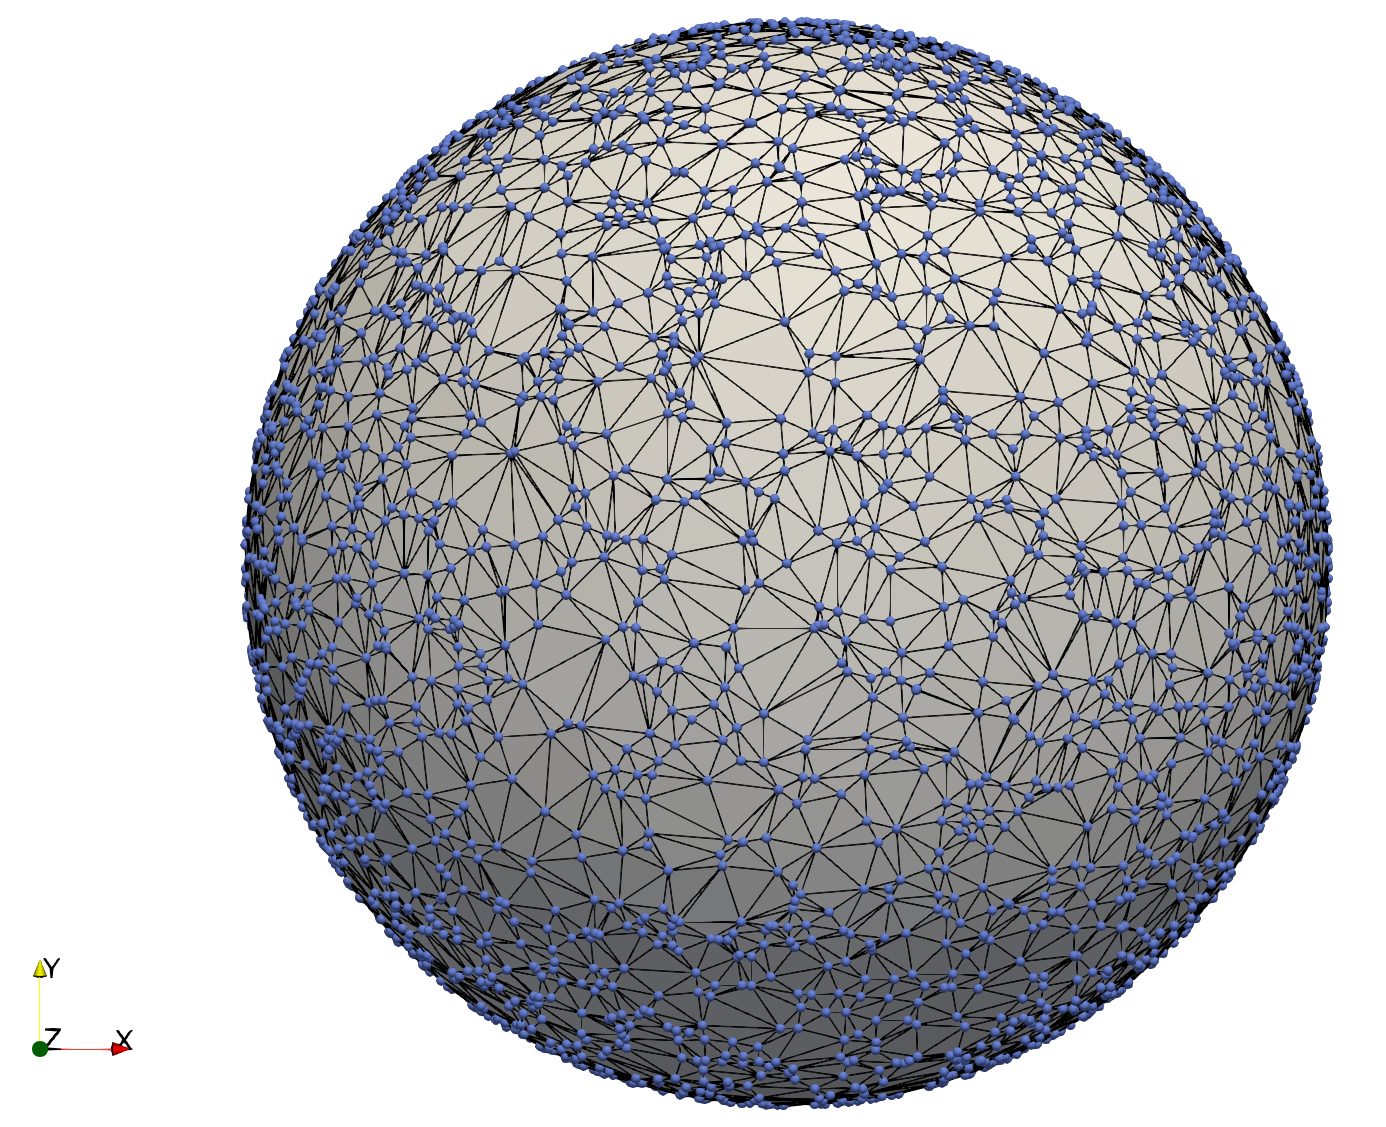
\includegraphics[width=0.4\textwidth,height=\textheight]{figs/surf_mc_random.png}
  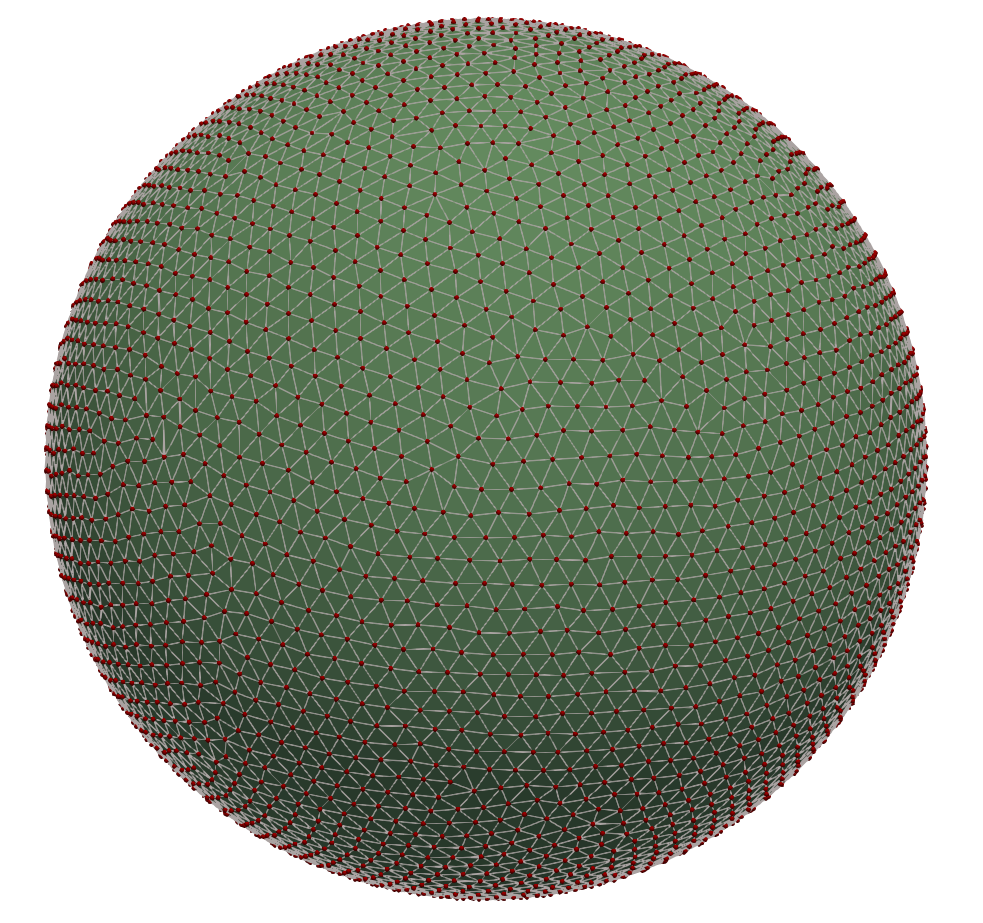
\includegraphics[width=0.4\textwidth,height=\textheight]{figs/surf_mc_lattice.png}
  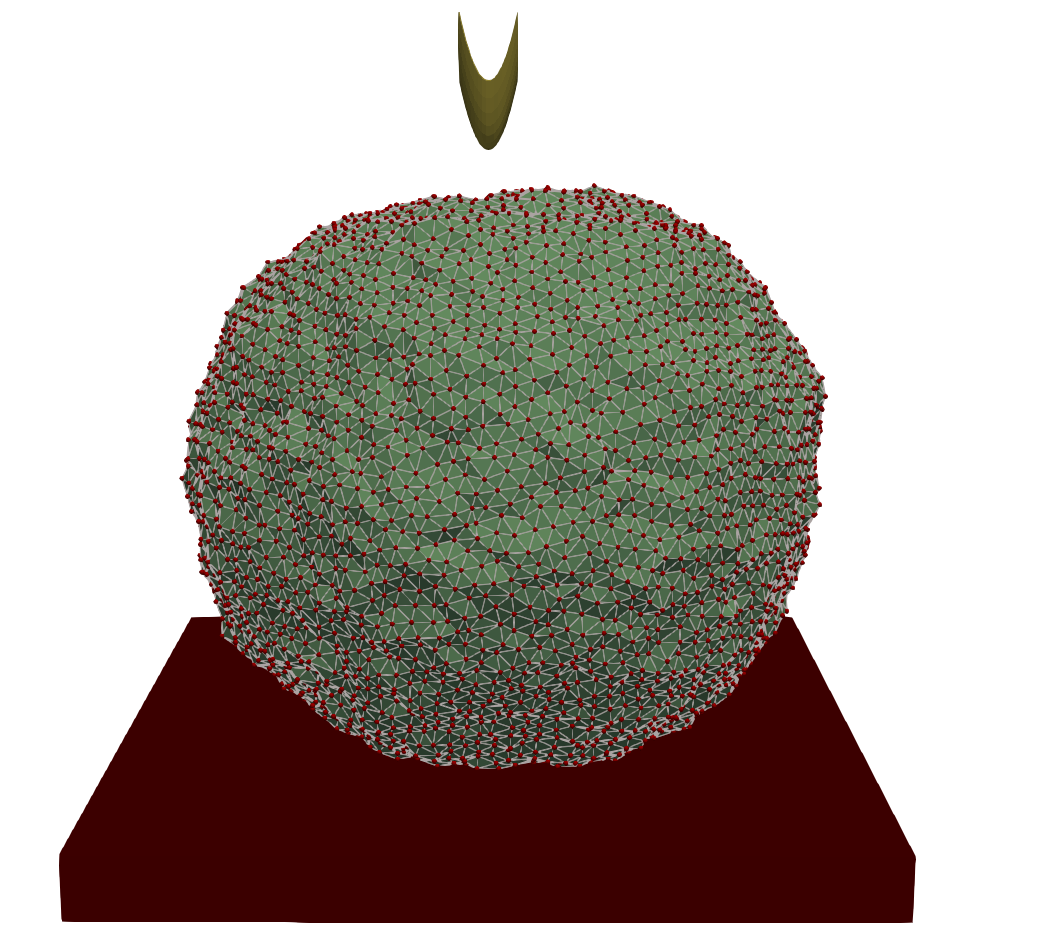
\includegraphics[width=0.4\textwidth,height=\textheight]{figs/tip_1p05.png}
  \label{fig:surf_mc}
  \caption{We perform monte-carlo simulation on the surface of sphere to generate equidistant points. \textbf{(A)} Random points on sphere ($Np=5120$, where $Np$ is number of points on the surface. \textbf{(B)} Points on the sphere after 60000 iteration of surface monte carlo simulation. We use Spherical-Voronoi to triangulate the mesh.}
\end{figure}
\begin{figure}
  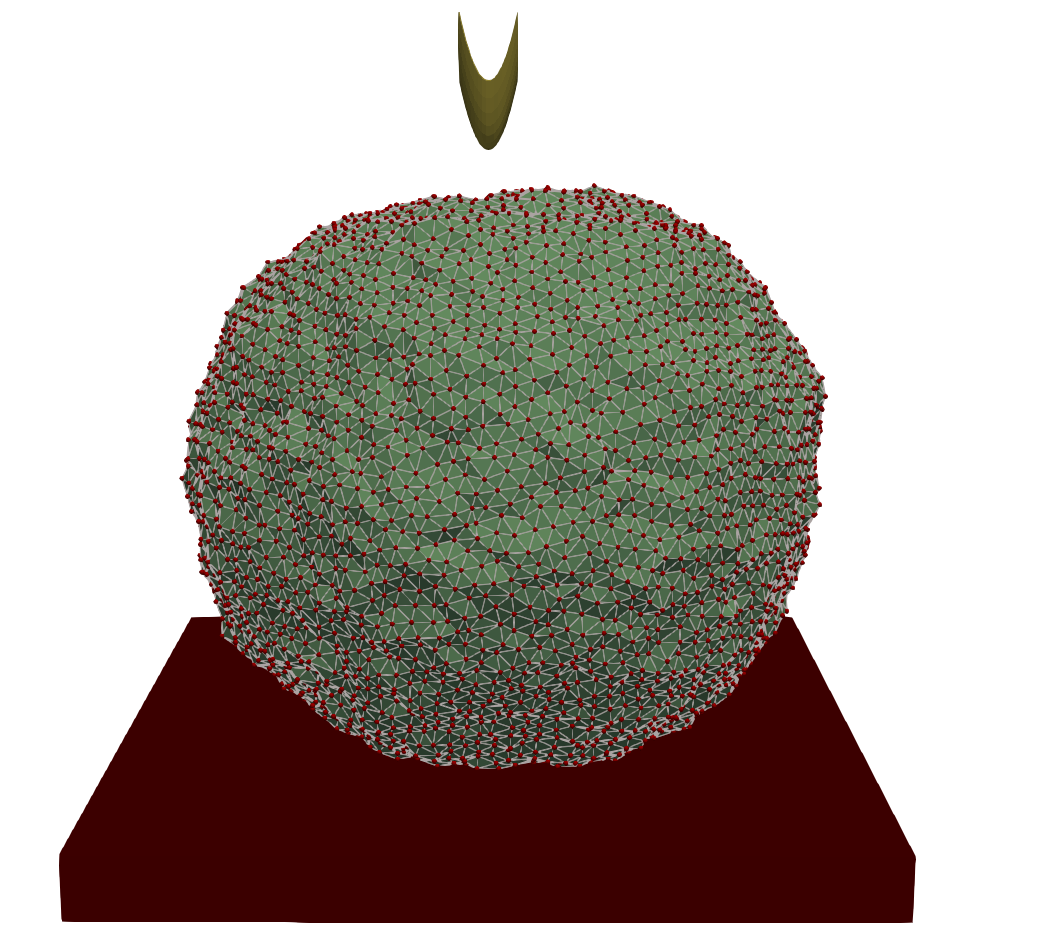
\includegraphics[width=0.32\textwidth,height=\textheight]{figs/tip_1p05.png}
  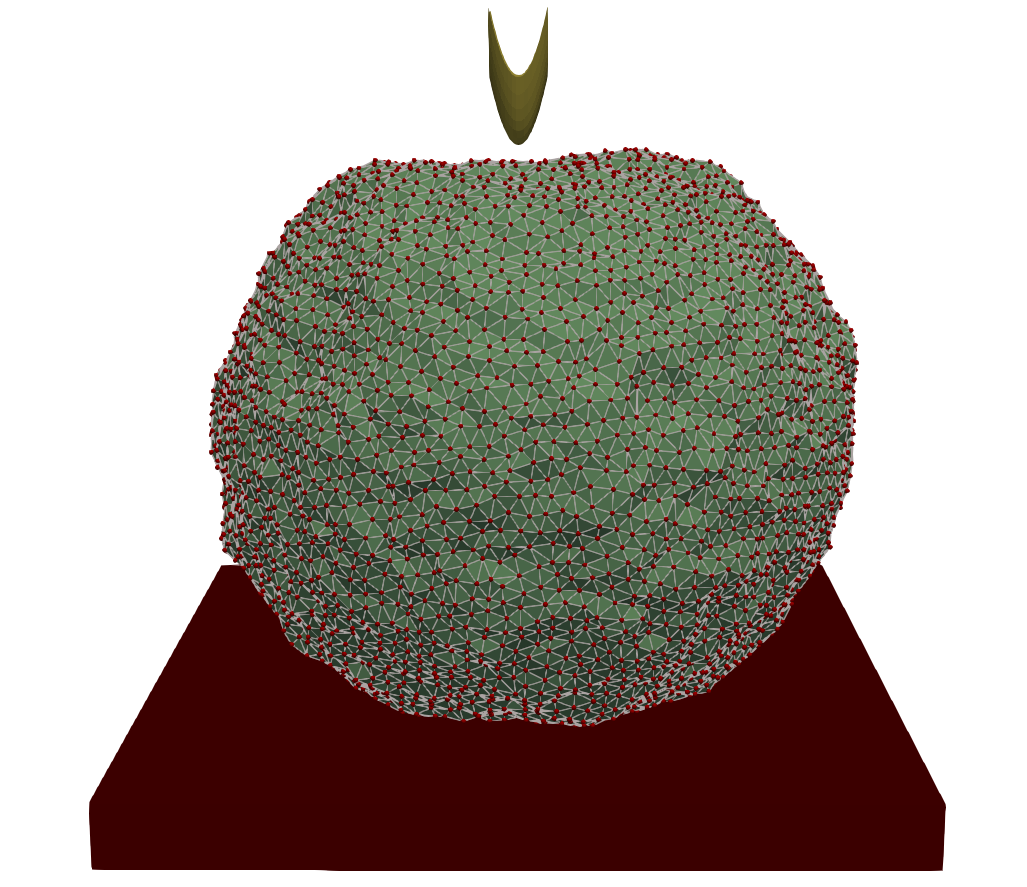
\includegraphics[width=0.32\textwidth,height=\textheight]{figs/tip_0p9.png}
  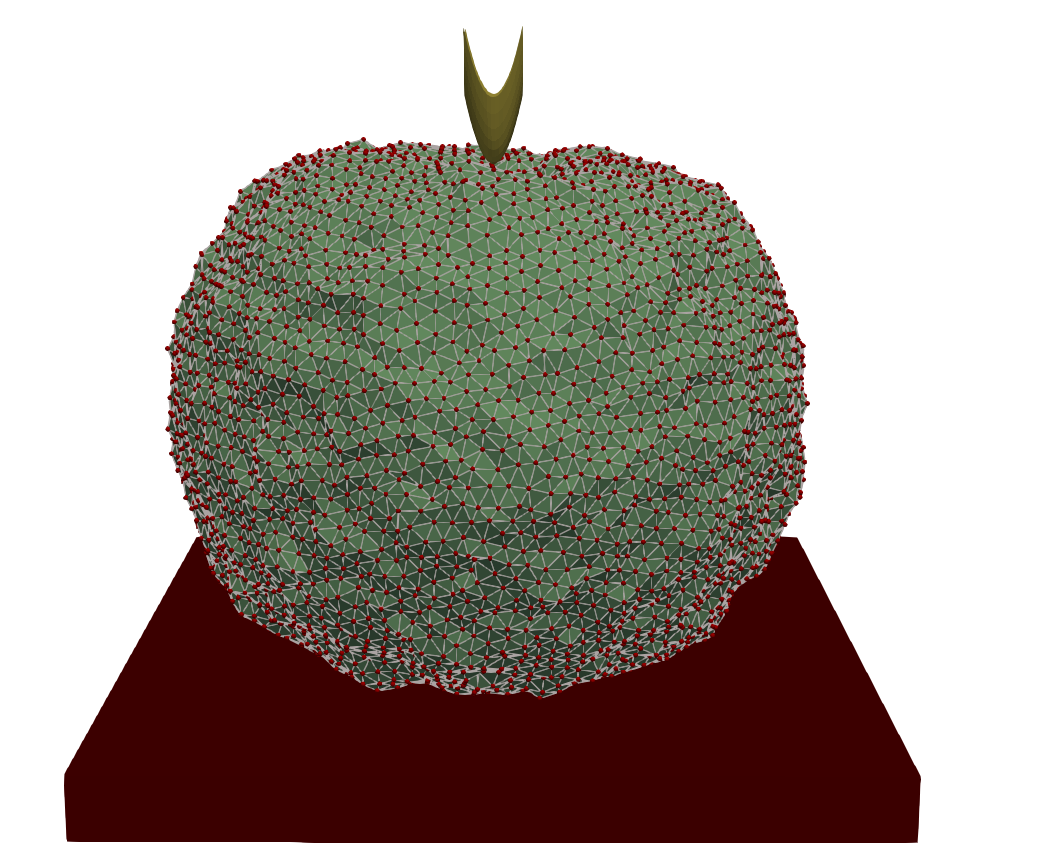
\includegraphics[width=0.32\textwidth,height=\textheight]{figs/tip_0p75.png}
  \label{fig:push_tip}
  \caption{Here we illustrate the shape of spherical membrane, if we push it from the top using an AFM tip. The membrane is stuck to the bottom by using attractive part of $LJ$ potential. \textbf{(A)} $t_z = 1.05R$, where $t_z$ is the tip position and $R$ is radius of the sphere. \textbf{(B)} $t_z = 0.9R$ and \textbf{(C)} $t_z = 0.75R$}
\end{figure}
\end{document}